\section{Hyper Text Transfer Protocol}

Web pages are composed of multiple resources which are uniquely identified by a Uniform Resource Locator (URL) or a Uniform Resource Identifier (URI).
When a client requests a resource using a URL, the request is resolved through Domain Name Resolution (DNS), followed by the retrieval of the requested data from the corresponding web server.

On the web, resources are managed by servers, identified through URIs, and accessed synchronously by clients using a request and response paradigm.
This model aligns with the REpresentational State Transfer (REST) architectural style.

\subsection{Communication}
HTTP follows a client-server architecture, where communication occurs as follows:
\begin{itemize}
    \item The client sends an HTTP request for a specific resource, identified by its URI.
    \item The server processes the request and responds with the requested resource or an appropriate status message.
\end{itemize}
\noindent HTTP is a stateless protocol, meaning each request is independent, and the server does not retain memory of previous interactions. 

\paragraph*{Requests}
HTTP requests are ASCII-encoded and follow a format that includes various fields.
\begin{figure}[H]
    \centering
    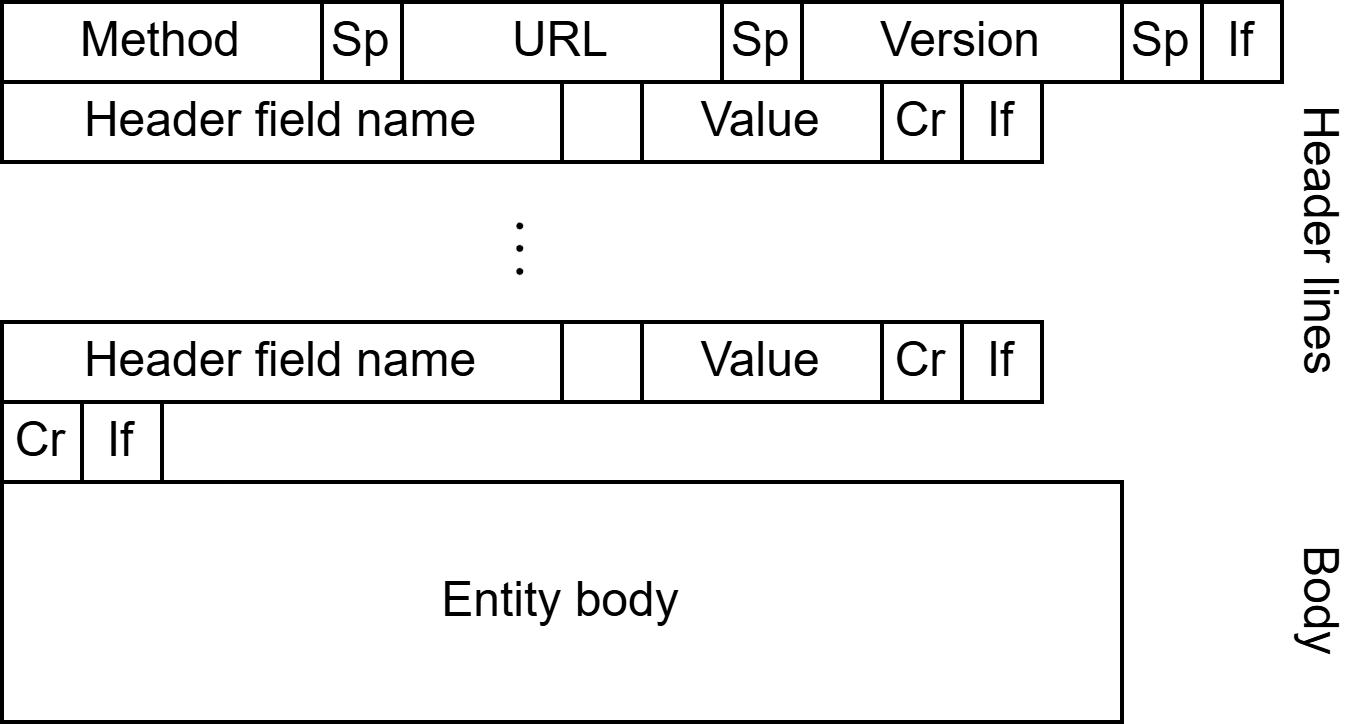
\includegraphics[width=0.5\linewidth]{images/iot7.png}
    \caption{HTTP request}
\end{figure}

\paragraph*{Responses}
HTTP responses follow a similar format, including a status code that indicates the outcome of the request:
\begin{itemize}
    \item \textit{Informational} (1xx): request received and processing continues.
    \item \textit{Success} (2xx): the request was successfully processed.
    \item \textit{Redirection} (3xx): further action is needed to complete the request.
    \item \textit{Client-side error} (4xx): the request contains incorrect syntax or cannot be fulfilled.
    \item \textit{Server-side error} (5xx): the server encountered an issue while processing the request.
\end{itemize}
\begin{figure}[H]
    \centering
    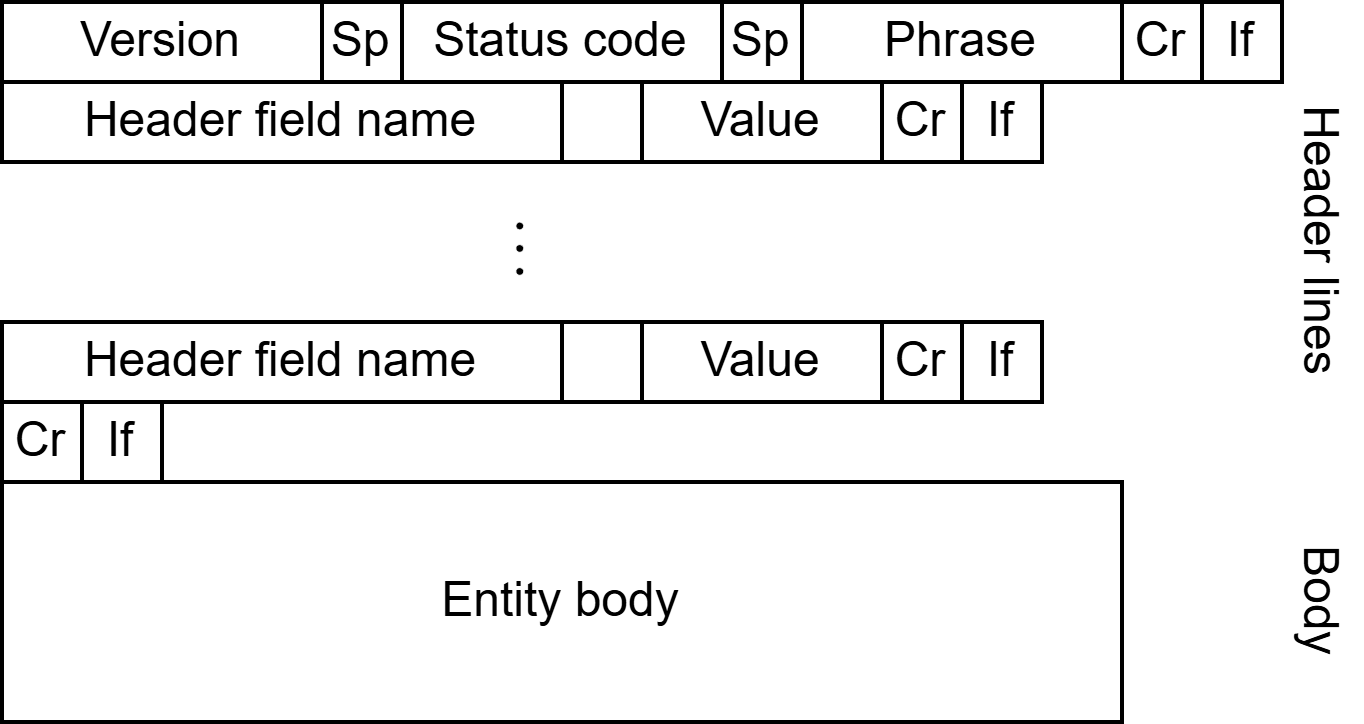
\includegraphics[width=0.5\linewidth]{images/iot8.png}
    \caption{HTTP response}
\end{figure}